% XeLaTex
\documentclass[tikz,border=3.14mm]{standalone}
\usetikzlibrary{shadings}
\usepackage{pgfplots}
\pgfplotsset{compat=1.16}
\usepackage{hyperref}

\begin{document}

reference: \url{https://tex.stackexchange.com/questions/479814/a-diagram-about-partial-derivatives-of-fx-y}

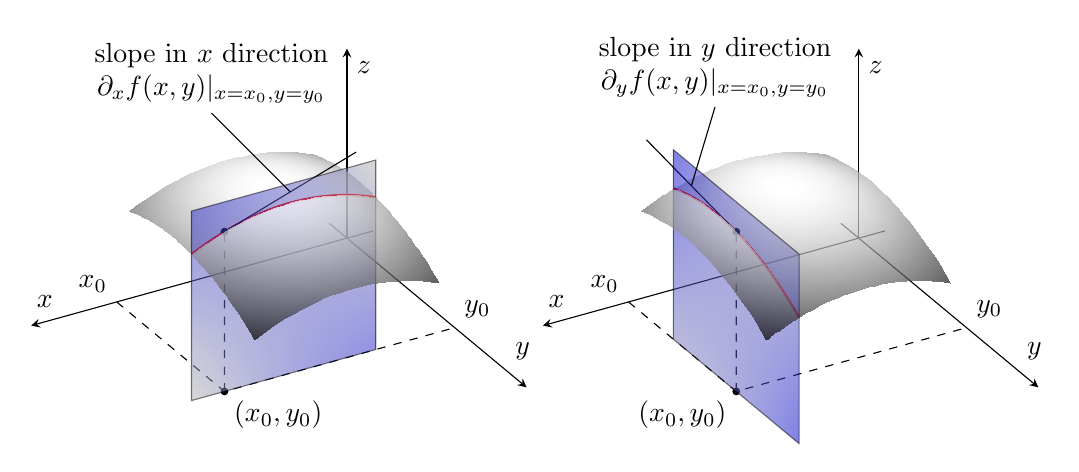
\begin{tikzpicture}[bullet/.style={circle,fill,inner sep=1pt},
 declare function={f(\x,\y)=2-0.5*pow(\x-1.25,2)-0.5*pow(\y-1,2);}]
 \begin{axis}[view={150}{45},colormap/blackwhite,axis lines=middle,%
    zmax=2.2,zmin=0,xmin=-0.2,xmax=2.4,ymin=-0.2,ymax=2,%
    xlabel=$x$,ylabel=$y$,zlabel=$z$,
    xtick=\empty,ytick=\empty,ztick=\empty]
  \addplot3[surf,shader=interp,domain=0.6:2,domain y=0.5:1.2,opacity=0.7] 
   {f(x,y)};
  \addplot3[thick,domain=0.6:2,samples y=1,color=red]  ({x},1.2,{f(x,1.2)}); 
  \draw[dashed] (1.75,0,0) node[above left]{$x_0$} -- (1.75,1.2,0)
  node[bullet] (b1) {}  -- (0,1.2,0) node[above right]{$y_0$}
  (1.75,1.2,0) -- (1.75,1.2,{f(1.75,1.2)})node[bullet] {};
  \draw (1.75,1.2,{f(1.75,1.2)}) -- (0.75,1.2,{f(1.75,1.2)+0.5})
  coordinate[pos=0.5] (aux1);
  \draw[opacity=0.5,upper left=blue!80!black,upper right=gray!60,
lower left=gray!60,lower right=blue!80!black] (2,1.2,0) -- (0.6,1.2,0)
   -- (0.6,1.2,2.2) -- (2,1.2,2.2) -- cycle;
  \addplot3[surf,shader=interp,domain=0.6:2,domain y=1.2:1.9,opacity=0.7] 
   {f(x,y)};
 \end{axis}
 
 \draw (aux1) -- ++ (-1,1) node[above,align=center]{slope in $x$ direction\\
  $\partial_xf(x,y)|_{x=x_0,y=y_0}$};
 \node[anchor=north west] at (b1) {$(x_0,y_0)$}; 
 %
 \begin{axis}[xshift=6.5cm,view={150}{45},colormap/blackwhite,axis lines=middle,%
    zmax=2.2,zmin=0,xmin=-0.2,xmax=2.4,ymin=-0.2,ymax=2,%
    xlabel=$x$,ylabel=$y$,zlabel=$z$,
    xtick=\empty,ytick=\empty,ztick=\empty]
  \addplot3[surf,shader=interp,domain=0.6:1.75,domain y=0.5:1.9,opacity=0.7] 
   {f(x,y)};
   \addplot3[thick,domain=0.5:1.9,samples y=1,color=red]  (1.75,{x},{f(1.75,x)}); 
  \draw[dashed] (1.75,0,0) node[above left]{$x_0$} -- (1.75,1.2,0)
  node[bullet] (b2){}
  -- (0,1.2,0) node[above right]{$y_0$}
  (1.75,1.2,0) -- (1.75,1.2,{f(1.75,1.2)})node[bullet] {};
  \draw (1.75,1.2,{f(1.75,1.2)}) -- (1.75,0.2,{f(1.75,1.2)+0.2})
   coordinate[pos=0.5] (aux2);
  \draw[opacity=0.5,upper left=blue!80!black,upper right=gray!60,
lower left=gray!60,lower right=blue!80!black] (1.75,0.5,0) -- (1.75,1.9,0)
   -- (1.75,1.9,2.2) -- (1.75,0.5,2.2) -- cycle;
  \addplot3[surf,shader=interp,domain=1.75:2,domain y=0.5:1.9,opacity=0.7] 
   {f(x,y)};
 \end{axis}
 \draw (aux2) -- ++ (0.3,1) node[above,align=center]{slope in $y$ direction\\
  $\partial_yf(x,y)|_{x=x_0,y=y_0}$};
 \node[anchor=north east] at (b2) {$(x_0,y_0)$};
\end{tikzpicture}
\end{document}